\section{Theory}
%%%%%%%%%%%%%%%%%%%%%%%%%%%%%%%%%%%%%%%%%%%%%%%%%%%%%%%%%%%%%%%%%%%%
\begin{frame}[fragile, c]
  \frametitle{Theory: Basic Idea of N-Body Simulations}
  The goal of an n-body simulation is to establish equations of motion for each body.
  
  \begin{center}
  \vspace*{-1em}
  \begin{tikzpicture}
  \coordinate (origo) at (0,0);
  \node[below=0.1 of origo] {$(0, 0, 0)$};
  
  % body 1
  \node[shading=ball,circle,minimum size=0.5cm,ball color=ForestGreen!80!white] at (5,5) (m1) {$m_1$};
  \draw [dotted,->] (origo) -- (m1) node[midway,sloped,below] {$\vec{r}_1$};
  \draw [dashed,thick,->,ForestGreen] (m1) -- ++(-1,1)  node[midway,sloped,above] {$\vec{v}_1$};
  \draw [dashed,thick,->,NavyBlue] (m1) -- ++(-0.8,-0.2) node[sloped,near end,anchor=east] {$\vec{a}_{1,2}$};
  \draw [dashed,thick,->,orange] (m1) -- ++(0.4,-0.6) node[sloped,near end,anchor=west] {$\vec{a}_{1,3}$};
  \draw [dashed,->,NavyBlue!60] (m1) ++(-1,1)  --  ++(-0.8,-0.2);
  \draw [dashed,->,orange!60] (m1) ++(-1.8,0.8)  --  ++(0.4,-0.6);
  \draw [very thick,->,red] (m1)   --  ++(-1.4,0.2);
  
  % body 2
  \node[shading=ball,circle,minimum size=0.5cm,ball color=NavyBlue!80!white] at (-3,3) (m2) {$m_2$};
  \draw [dotted,->] (origo) -- (m2) node[midway,sloped,below] {$\vec{r}_2$};
  \draw [dashed,thick,->,NavyBlue] (m2) -- ++(1,1.3)  node[midway,sloped,above] {$\vec{v}_2$};
  \draw [dashed,thick,->,ForestGreen] (m2) -- ++(0.8,0.2) node[sloped,near end,anchor=west] {$\vec{a}_{2,1}$};
  \draw [dashed,thick,->,orange] (m2) -- ++(1,-0.1) node[sloped,near end,anchor=west] {$\vec{a}_{2,3}$};
  \draw [dashed,->,ForestGreen!60] (m2)++(1,1.3) -- ++(0.8,0.2);
  \draw [dashed,->,orange!60] (m2)++(1.8,1.5) -- ++(1,-0.1);
  \draw [very thick,->,red] (m2) -- ++(2.8,1.4);
  
  % body 3
  \node[shading=ball,circle,minimum size=0.5cm,ball color=orange!80!white] at (7,2) (m3) {$m_3$};
  \draw [dotted,->] (origo) -- (m3) node[midway,sloped,below] {$\vec{r}_3$};
  \draw [dashed,thick,->,orange] (m3) -- ++(0.8,0.9)  node[midway,sloped,above] {$\vec{v}_3$};
  \draw [dashed,thick,->,ForestGreen] (m3) -- ++(-0.4,0.6) node[sloped,near end, anchor=east] {$\vec{a}_{3,1}$};
  \draw [dashed,thick,->,NavyBlue] (m3) -- ++(-1,0.1) node[sloped, near end, anchor=east] {$\vec{a}_{3,2}$};
  \draw [dashed,->,ForestGreen!60] (m3)++(0.8,0.9) -- ++(-0.4,0.6);
  \draw [dashed,->,NavyBlue!60] (m3)++(0.4,1.5) --  ++(-1,0.1);
  \draw [very thick,->,red] (m3) -- ++(-0.6,1.6);
  \end{tikzpicture}
  \end{center}
\end{frame}
%%%%%%%%%%%%%%%%%%%%%%%%%%%%%%%%%%%%%%%%%%%%%%%%%%%%%%%%%%%%%%%%%%%%

%%%%%%%%%%%%%%%%%%%%%%%%%%%%%%%%%%%%%%%%%%%%%%%%%%%%%%%%%%%%%%%%%%%%
\begin{frame}[fragile]
  \frametitle{Theory: Naive Formulation of an N-Body Simulation Problem}
  Each body $i$ with its mass $m_i$ and position vector $\vec{r}_i$ experiences the force $\vec{a}_i$ from all other bodies according to Newton's law of universal gravitation:
  \begin{equation*}
    \vec{a}_i = \sum\limits_{i \neq j} G m_j \frac{\vec{r}_j - \vec{r}_i}{(\norm{\vec{r}_j - \vec{r}_i}_2^2 + \epsilon^2)^\frac{3}{2}}
  \end{equation*}
  \pause
  \begin{itemize}
    \item gravitational constant: $G = \num{6.67430e-11}\frac{\text{m}^3}{\text{kg} \cdot \text{s}^2}$
    \item The physical units of $G$ do not reflect the units used in the data sets:
          \begin{itemize}
            \item distance in astronomical units:  $\SI{1}{\au} = \SI{1.49597870691e+11}{\meter}$
            \item time in days: $\SI{1}{\day} = \SI{86400}{\second}$
          \end{itemize}
    \item \textbf{Note:} the correctly scaled $G$ should be calculate in your program!
    \item softening factor: $\epsilon = \num{1e-11}$ to prevent collisions between two bodies
    \item $\norm{}_2^2$: squared Euclidean distance
  \end{itemize}
\end{frame}
%%%%%%%%%%%%%%%%%%%%%%%%%%%%%%%%%%%%%%%%%%%%%%%%%%%%%%%%%%%%%%%%%%%%

%%%%%%%%%%%%%%%%%%%%%%%%%%%%%%%%%%%%%%%%%%%%%%%%%%%%%%%%%%%%%%%%%%%%
\begin{frame}[fragile]
  \frametitle{Theory: Energy of the System}
  \begin{itemize}
    \item kinetic energy: $E_K = \sum\limits_{i}\frac{1}{2} m_i \norm{\vec{v}_i}_2^2$
    \item potential energy: $E_P = -\sum\limits_{i < j} \frac{G m_i m_j}{\norm{\vec{r}_j - \vec{r}_i}_2}$
    \item sum of the energies in the system: $E_T = E_K + E_P$\vspace{.7em}
    \item $E_T$ must be \enquote{constant} in a stable simulation (conservation of energy)!
  \end{itemize}
  \vfill
  \pause
  The Virial Equilibrium:
  
  $$ \frac{2 \cdot E_K}{\abs{E_P}} \approx 1.0 $$
  
  as a dynamic equilibrium state on a timescale comparable to a few times the typical time needed for a body to cross the system.
  \vfill
  \textbf{Question:} What happens if the result is $> 1.0$ or $< 1.0$?
  
  \vfill
  \setfontsize{8pt}
  See: \url{http://www.scholarpedia.org/article/N-body_simulations_(gravitational)}
\end{frame}
%%%%%%%%%%%%%%%%%%%%%%%%%%%%%%%%%%%%%%%%%%%%%%%%%%%%%%%%%%%%%%%%%%%%

\subsection{Barnes-Hut}
%%%%%%%%%%%%%%%%%%%%%%%%%%%%%%%%%%%%%%%%%%%%%%%%%%%%%%%%%%%%%%%%%%%%
\begin{frame}[fragile]
  \frametitle{Theory: Barnes-Hut Algorithm to Speed Up the Simulation}
  Combine bodies that are far enough away from pseudo-bodies to reduce the number of necessary force calculations.
  \vfill
  \begin{center}
  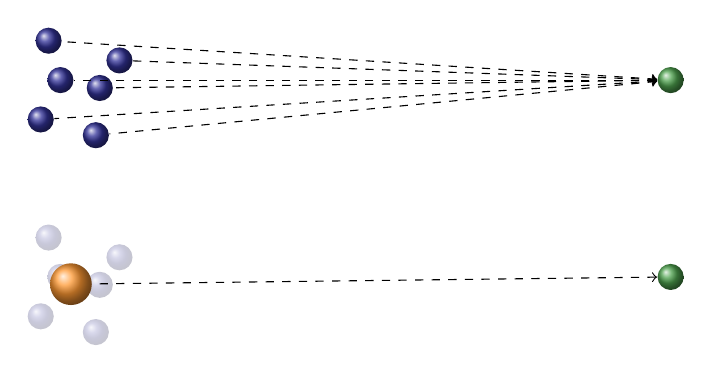
\begin{tikzpicture}
  \begin{scope}
      \node[shading=ball,circle,ball color=NavyBlue!80!white] at (0, 0) (m0) {};
      \node[shading=ball,circle,ball color=NavyBlue!80!white] at (1, 0.75) (m1) {};
      \node[shading=ball,circle,ball color=NavyBlue!80!white] at (.25, 0.5) (m2) {};
      \node[shading=ball,circle,ball color=NavyBlue!80!white] at (0.1, 1) (m3) {};
      \node[shading=ball,circle,ball color=NavyBlue!80!white] at (.75, .4) (m4) {};
      \node[shading=ball,circle,ball color=NavyBlue!80!white] at (.7, -.2) (m5) {};
      
      \node[shading=ball,circle,ball color=ForestGreen!80!white] at (8, .5) (mm) {};
      
      \foreach \x in {0,...,5}
        \draw[dashed, <-] (mm) edge (m\x);
  \end{scope}
  \begin{scope}[shift={(0, -2.5)}]
      \node[shading=ball,circle,ball color=NavyBlue!80!white,opacity=.25] at (0, 0) (m0) {};
      \node[shading=ball,circle,ball color=NavyBlue!80!white,opacity=.25] at (1, 0.75) (m1) {};
      \node[shading=ball,circle,ball color=NavyBlue!80!white,opacity=.25] at (.25, 0.5) (m2) {};
      \node[shading=ball,circle,ball color=NavyBlue!80!white,opacity=.25] at (0.1, 1) (m3) {};
      \node[shading=ball,circle,ball color=NavyBlue!80!white,opacity=.25] at (.75, .4) (m4) {};
      \node[shading=ball,circle,ball color=NavyBlue!80!white,opacity=.25] at (.7, -.2) (m5) {};
      
      \node[shading=ball,circle,scale=1.6,ball color=orange!80!white] at (.3833, .4083) (mcof) {};
  
      \node[shading=ball,circle,ball color=ForestGreen!80!white] at (8, .5) (mm) {};
      
      \draw[dashed, <-] (mm) edge (mcof);
  \end{scope}
  \begin{scope}[overlay]
    \draw[dotted, ->] (-.9, .4803) to [out=210,in=150] (-.9, .4803 + -2.5);
    \node[rotate=90] at (-1.8, .4803 + (-2.5 / 2) {\scriptsize approximation};
  \end{scope}
  \end{tikzpicture}
  \end{center}
  \vfill
  \setfontsize{8pt}
  See: \texttt{Josh Barnes and Piet Hut: A hierarchical O(N log N) force-calculation algorithm (1986)\\[-.5em]
  (DOI: \url{https://doi.org/10.1038/324446a0})}
\end{frame}
%%%%%%%%%%%%%%%%%%%%%%%%%%%%%%%%%%%%%%%%%%%%%%%%%%%%%%%%%%%%%%%%%%%%

%%%%%%%%%%%%%%%%%%%%%%%%%%%%%%%%%%%%%%%%%%%%%%%%%%%%%%%%%%%%%%%%%%%%
\begin{frame}[fragile]
  \frametitle{Theory: Barnes-Hut - Example: Quadtree}
  \begin{tikzpicture}
    \begin{scope}[scale=0.9]
        % Quadtree grid
        \draw[step=4] (0, 0) grid (8, 8);
        
        \draw[step=2] (0, 0) grid (4, 4);
        \draw[step=2] (4, 4) grid (8, 8);
        \draw[step=2] (4, 0) grid (8, 4);
        
        \draw[step=1] (0, 0) grid (2, 2);
        \draw[step=1] (0, 2) grid (2, 4);
        \draw[step=1] (2, 0) grid (4, 2);
        \draw[step=1] (4, 4) grid (6, 6);
        \draw[step=1] (6, 4) grid (8, 6);
        
        \draw[thick,orange] (0, 0) rectangle (4, 4);
        
        
        % bodies
        % top left
        
        % top right
        % 1.337
        \node[shading=ball,circle,ball color=NavyBlue!80!white] (p1) at (4.35, 4.4) {};
        \node[shading=ball,circle,ball color=NavyBlue!80!white] (p2) at (4.5, 5.4) {};
        \node[shading=ball,circle,ball color=NavyBlue!80!white] (p3) at (5.6, 4.7) {};
        
        \node[shading=ball,circle,ball color=ForestGreen!80!white] (p) at (6.3, 4.65) {};
        \node[shading=ball,circle,ball color=NavyBlue!80!white] (p4) at (6.4, 5.25) {};
        \node[shading=ball,circle,ball color=NavyBlue!80!white] (p5) at (7.5, 7.5) {};
        
        % bottom left
        \node[shading=ball,circle,ball color=NavyBlue!80!white,opacity=.25] at (1.5, 1.5) {};
        \node[shading=ball,circle,ball color=NavyBlue!80!white,opacity=.25] at (0.6, 0.7) {};
        \node[shading=ball,circle,ball color=NavyBlue!80!white,opacity=.25] at (1.4, 2.3) {};
        \node[shading=ball,circle,ball color=NavyBlue!80!white,opacity=.25] at (0.75, 2.4) {};
        \node[shading=ball,circle,ball color=NavyBlue!80!white,opacity=.25] at (1.3, 0.75) {};
        \node[shading=ball,circle,ball color=NavyBlue!80!white,opacity=.25] at (2.22, 0.78) {};
        \node[shading=ball,circle,ball color=NavyBlue!80!white,opacity=.25] at (2.4, 1.3) {};
        
        % center of mass of distant bodies
        \node[shading=ball,circle,scale=1.7,ball color=orange!80!white] (pp) at (1.45, 1.39) {}; % 0.6844
        
        % bottom right % 1.821
        \node[shading=ball,circle,ball color=NavyBlue!80!white] (p6) at (7.5, 1.75) {}; % 0.637
        \node[shading=ball,circle,ball color=NavyBlue!80!white] (p7) at (6.8, 3.5) {}; % 1.594
        
        
        % theta
        \draw[thick,dashed,<-] (p) -- (pp) node[midway, pos=.3, below] {$\vec{d}$};
        \draw [decorate,decoration={brace,amplitude=10pt,raise=4pt}] (0.01, 4) -- (3.99, 4) node [midway,yshift=.7cm] {\small edge length};
        \foreach \x in {1,...,7}
            \draw[dotted,<-] (p) -- (p\x);
    \end{scope}
    
    \begin{scope}[overlay, scale=0.9]
        \node[align=left,text width=5cm] (nt) at (12.5, 7.5) {Use pseudo-bodies to calculate the forces if:};
        \node[align=center, below=-.1cm of nt] {$\dfrac{\text{edge length}}{\norm{\vec{d}}_2} < \theta$};
    \end{scope}
    \begin{scope}[shift={(8, -1.5)}, scale=0.95]
        \node[shading=ball,circle,scale=2.5,ball color=orange!80!white,opacity=.25] (root) at (3.1, 6) {};
        
        % top right
        \node[shading=ball,circle,scale=1.6,ball color=orange!80!white,opacity=.25] (l11) at (1, 5) {};
        \node[shading=ball,circle,ball color=NavyBlue!80!white] (l21) at (0.3, 4) {};
        \node[shading=ball,circle,scale=1.2,ball color=orange!80!white,opacity=.25] (l22) at (1, 4) {};
        \node[shading=ball,circle,ball color=NavyBlue!80!white] (l31) at (0.8, 3) {};
        \node[shading=ball,circle,ball color=ForestGreen!80!white] (l32) at (1.2, 3) {};
        \node[shading=ball,circle,scale=1.3,ball color=orange!80!white,opacity=.25] (l23) at (2, 4) {};
        \node[shading=ball,circle,ball color=NavyBlue!80!white] (l33) at (1.6, 3) {};
        \node[shading=ball,circle,ball color=NavyBlue!80!white] (l34) at (2, 3) {};
        \node[shading=ball,circle,ball color=NavyBlue!80!white] (l35) at (2.4, 3) {};
        
        \draw[thick] (root) -- (l11);
        \draw[thick] (l11) -- (l21);
        \draw[thick] (l11) -- (l22);
        \draw[thick] (l11) -- (l23);
        \draw[thick] (l22) -- (l31);
        \draw[thick] (l22) -- (l32);
        \draw[thick] (l23) -- (l33);
        \draw[thick] (l23) -- (l34);
        \draw[thick] (l23) -- (l35);
        
        % bottom right
        \node[shading=ball,circle,scale=1.2,ball color=orange!80!white,opacity=.25] (l12) at (3.1, 5) {};
        \node[shading=ball,circle,ball color=NavyBlue!80!white] (l24) at (2.8, 4) {};
        \node[shading=ball,circle,ball color=NavyBlue!80!white] (l25) at (3.4, 4) {};
        \draw[thick] (root) -- (l12);
        \draw[thick] (l12) -- (l24);
        \draw[thick] (l12) -- (l25);
        
        % bottom left
        \node[shading=ball,circle,scale=1.7,ball color=orange!80!white] (l13) at (5.2, 5) {};
        \node[shading=ball,circle,scale=1.2,ball color=orange!80!white,opacity=.25] (l26) at (4.2, 4) {};
        \node[shading=ball,circle,ball color=NavyBlue!80!white,opacity=.25] (l36) at (4.4, 3) {};
        \node[shading=ball,circle,ball color=NavyBlue!80!white,opacity=.25] (l37) at (4, 3) {};
        \node[shading=ball,circle,scale=1.3,ball color=orange!80!white,opacity=.25] (l27) at (5.2, 4) {};
        \node[shading=ball,circle,ball color=NavyBlue!80!white,opacity=.25] (l38) at (4.8, 3) {};
        \node[shading=ball,circle,ball color=NavyBlue!80!white,opacity=.25] (l39) at (5.2, 3) {};
        \node[shading=ball,circle,ball color=NavyBlue!80!white,opacity=.25] (l310) at (5.6, 3) {};
        \node[shading=ball,circle,scale=1.2,ball color=orange!80!white,opacity=.25] (l28) at (6.2, 4) {};
        \node[shading=ball,circle,ball color=NavyBlue!80!white,opacity=.25] (l311) at (6, 3) {};
        \node[shading=ball,circle,ball color=NavyBlue!80!white,opacity=.25] (l312) at (6.4, 3) {};
        \draw[thick] (root) -- (l13);
        \draw[thick,opacity=.25] (l13) -- (l26);
        \draw[thick,opacity=.25] (l13) -- (l27);
        \draw[thick,opacity=.25] (l13) -- (l28);
        \draw[thick,opacity=.25] (l26) -- (l36);
        \draw[thick,opacity=.25] (l26) -- (l37);
        \draw[thick,opacity=.25] (l27) -- (l38);
        \draw[thick,opacity=.25] (l27) -- (l39);
        \draw[thick,opacity=.25] (l27) -- (l310);
        \draw[thick,opacity=.25] (l28) -- (l311);
        \draw[thick,opacity=.25] (l28) -- (l312);
        
        \node[anchor=west] at (0, 2.2) {\small naive: $\num{14}$ force calculations};
        \node[anchor=west] at (0, 1.7) {\small Barnes-Hut: $\num{8}$ force calculations};
    \end{scope}
  \end{tikzpicture}
\end{frame}
%%%%%%%%%%%%%%%%%%%%%%%%%%%%%%%%%%%%%%%%%%%%%%%%%%%%%%%%%%%%%%%%%%%%

%%%%%%%%%%%%%%%%%%%%%%%%%%%%%%%%%%%%%%%%%%%%%%%%%%%%%%%%%%%%%%%%%%%%
\begin{frame}[fragile]
  \frametitle{Theory: Barnes-Hut - Tree Node}
  Each node of the octree (extension of the quadtree for the $3$-dimensional space) has to save the following information:
  \begin{itemize}
      \item edge length of the octree-octant
      \item sum of the masses of all bodies in the octant: $m_{oct} = \sum_i m_i$
      \item center of mass of all bodies $i$ in the octant: $\vec{c}_{oct} = \dfrac{\sum_i m_i \vec{r}_i}{\sum_i m_i}$
      \item all children of the octant
  \end{itemize}
  \vfill
  Each leaf may only contain a single body!
\end{frame}
%%%%%%%%%%%%%%%%%%%%%%%%%%%%%%%%%%%%%%%%%%%%%%%%%%%%%%%%%%%%%%%%%%%%

%%%%%%%%%%%%%%%%%%%%%%%%%%%%%%%%%%%%%%%%%%%%%%%%%%%%%%%%%%%%%%%%%%%%
\begin{frame}[fragile]
  \frametitle{Theory: Barnes-Hut - Update the Accelerations $\vec{a}_i$}
  \begin{algorithmcl}
    \begin{algorithmic}[1]
        \Procedure{UpdateAcceleration}{\texttt{body}, \texttt{node}}
        \State{calculate direction vector $\vec{d}$ between \texttt{body} and the center of mass of \texttt{node}}
        \If{pseudo-body can be used $\vee$ \texttt{node} is leaf}
            \State{update acceleration of $\vec{a}_\text{\texttt{body}}$}
        \Else
            \For{each \texttt{child} of \texttt{node}}
                \State{\textsc{UpdateAcceleration}(\texttt{body}, \texttt{child})}
            \EndFor
        \EndIf
        \EndProcedure
    \end{algorithmic}
  \end{algorithmcl}
  \vfill
  \textbf{Question:}\\
  Is it also possible to speed up the force calculations using the Barnes-Hut tree?
\end{frame}
%%%%%%%%%%%%%%%%%%%%%%%%%%%%%%%%%%%%%%%%%%%%%%%%%%%%%%%%%%%%%%%%%%%%

\subsection{Time Stepping Method}
%%%%%%%%%%%%%%%%%%%%%%%%%%%%%%%%%%%%%%%%%%%%%%%%%%%%%%%%%%%%%%%%%%%%
\begin{frame}[fragile]
  \frametitle{Theory: Leapfrog Integration}
  The leapfrog integration, a 2nd order time step method, as a combination of the two variants of the symplectic Euler method (SE), is used to advance from the time step $k$ to the next time step $k + 1$:
  \begin{equation*}
    \begin{split}
      (SE1) &\left\lbrace
      \begin{array}{rcl}
        \vec{v}^{k+\frac{1}{2}} & = & \vec{v}^k + \vec{a}^k \frac{\Delta t}{2}               \\
        \vec{r}^{k+\frac{1}{2}} & = & \vec{r}^k + \vec{v}^{k + \frac{1}{2}} \frac{\Delta t}{2}
      \end{array}\right.\\[.5em]
      (SE2) &\left\lbrace
      \begin{array}{rcl}
        \vec{r}^{k+1} & = & \vec{r}^{k + \frac{1}{2}} + \vec{v}^{k + \frac{1}{2}} \frac{\Delta t}{2} \\
        \vec{v}^{k+1} & = & \vec{v}^{k + \frac{1}{2}} + \vec{a}^{k+1} \frac{\Delta t}{2}
      \end{array}\right.\\
    \end{split}
  \end{equation*} \\
  \vfill
  \setfontsize{8pt}
  See: \texttt{O. Buneman: Time-Reversible Difference Procedures (1967)\\[-.5em]
  (DOI: \url{https://doi.org/10.1016/0021-9991(67)90056-3})}
  % https://www.sciencedirect.com/science/article/pii/0021999167900563
  % https://www.sciencedirect.com/science/article/pii/0010465587900191
\end{frame}
%%%%%%%%%%%%%%%%%%%%%%%%%%%%%%%%%%%%%%%%%%%%%%%%%%%%%%%%%%%%%%%%%%%%

\subsection{Complete Simulation}
%%%%%%%%%%%%%%%%%%%%%%%%%%%%%%%%%%%%%%%%%%%%%%%%%%%%%%%%%%%%%%%%%%%%
\begin{frame}<1>[fragile, label={complete_simulation}]
  \frametitle<1>{Theory: A Complete Simulation}
  \frametitle<2>{A Complete Simulation}
\begin{algorithmcl}
    \begin{algorithmic}[1]
        \State{adjust initial velocities: $\vec{u}_i = \dfrac{\sum_j m_j \vec{v}_j}{\sum_j m_j}$;\quad$\vec{v}_i = \vec{v}_i - \vec{u}_i$}
        \State{update accelerations $\vec{a}_i$}
        \State{visualize initial state}
        \While{simulation not terminated yet}
            \State{perform leapfrog integration step}
            \If{time step should be visualized}
                \State{visualize time step}
            \EndIf
            \State{update time step}
        \EndWhile
        \State{Save final state of the simulation as \texttt{.csv} file (name + mass + positions + velocities)}
    \end{algorithmic}
\end{algorithmcl}
    \only<2>{\vfill\textbf{Question:} What can and should be parallelized?}
\end{frame}
%%%%%%%%%%%%%%%%%%%%%%%%%%%%%%%%%%%%%%%%%%%%%%%%%%%%%%%%%%%%%%%%%%%%
